\section{Signal Path}
\label{signPath}

The signal originates at the emitter. The for each pulse, the emitter position is determined from a
set of Kepler elements. The energy in the pulse is found by distributing the emitter power over a
constant number of pulses of a given duration.

The signal then starts to propagate through the atmosphere. The atmosphere effects the signal in
several manners, but the most important one (the only one that is also taken into account) is the
attenuation of the signal. The pulse energy exponentially decays with distance travel though the
atmosphere. Furthermore also the optical thickness of the atmosphere is a parameter in this process.

Then the intersection of the pulse with the \ac{DEM} is computed. As a simplification in this
process, the intersection of the pulse (ray) with a sphere with radius of the average terrain height
of the \ac{DEM} tile plus the earth radius is computed. Then the ray-sphere intersection point
coordinates are covered into latitude and longitude. These are then used to find the actual terrain
elevation from the \ac{DEM} and the 3d position.

Then the scattering characteristics are constructed by finding the terrain normal and the incidence
angle of the laser pulse. The power of the emitted pulse is now distributed over the entire
footprint area and then reflected back using the scattering technique described in section
\ref{scatter} (this is done for every satellite separately).

The reflected pulse now travels back trough the atmosphere. This causes more attenuation to take
place. The energy received by the receivers is now dependant on the receiver aperture. This received
energy can then converted into photons by dividing by the energy per photon.

\begin{figure}[ht!]
	\centering
		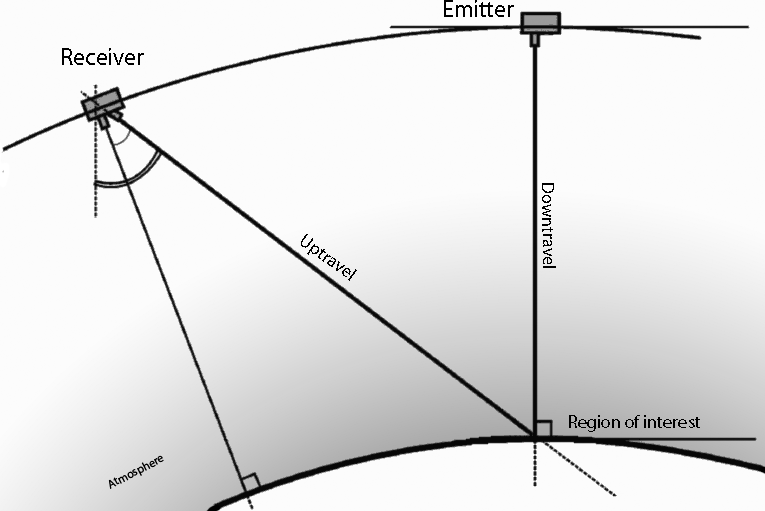
\includegraphics[width=0.4\textwidth]{chapters/img/signalPath.png}
		\label{fig:scatter}
	\caption{Signal path representation}
\end{figure}










